\chapter{Discussion}\label{ch:discussion}

This chapter discusses the obtained results and further possible improvements or extensions for the proposed solution.
First, it describes several ways the proposed solution can be improved or extended in section~\ref{sec:implementation}.


\section{Improvements and extensions}\label{sec:improvements}

\subsection{Free space}\label{subsec:free-space}

The extension of the proposed solution is to take a different approach to free space.
\definice{Free space} can be defined as a part of the painting placement solution where the painting is not placed.
For example, free space is important in the FLP problem as there is a need for an aisle between the facilities
through which the material transportation takes place~\cite{scholzExtensionsSTaTSPractical2010}.

In the proposed solution, two main parts influence where the free space is created.
It is (1) the placing heuristic and (2) the evaluation function $\pi$, see eq.~\ref{eq:objective}.
Placing heuristic works locally, i.e., only in the allocated area for the painting, and the evaluation
function, although it might be used to define arbitrary free space shape, is not a constraint but a penalization.
Thus, it does not guarantee that the painting placement solution will create a solution with the desired free space.

One possible approach to guarantee free space is the introduction of dummy paintings.
These dummy paintings can be injected during the slicing tree construction.
The resulting painting placement solution will thus, among the paintings, contain free space occupied by dummy paintings.

An example of dummy painting injection can be seen in figure~\ref{fig:dummy-painting}.
The aisle is created between paintings 1,2, and 3 by adding a vertical cut $V$ to the tree.


\begin{figure}[h!]
    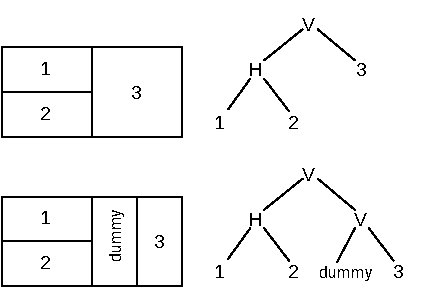
\includegraphics[height=0.33\textheight, center]{dummy_painting}
    \caption{Example of dummy painting injection.}
    \label{fig:dummy-painting}
\end{figure}

\subsection{Non-rectangular layouts}\label{subsec:non-rectangular-layouts}

Another extension to the proposed solution is adding the ability to work with layouts that are not rectangular.
It can be solved using the dummy paintings described in subsection~\ref{subsec:free-space}.
These dummy paintings are as small as possible and placed over the parts of the layout that are not rectangular.
By placing these dummy facilities, the layout becomes rectangular.
A similar approach is used in~\ref{scholzExtensionsSTaTSPractical2010} to modify a slicing tree to solve FLP.

An example of using dummy paintings to work with a non-rectangular layout is in figure~\ref{fig:non-rectangular-layout}.
There are two irregularities in both corners of the layout.
Two dummy paintings are injected into the slicing tree using a dummy painting injection to fill the irregularities.

\begin{figure}[h!]
    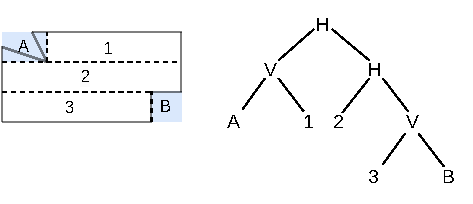
\includegraphics[width=0.8\textwidth, center]{non-rectangular-layout}
    \caption[Example of working with non-rectangular layout.]{Example of working with non-rectangular layout. The allocated area is marked using a dotted line.
    Dummy paintings that fill the irregularities in both corners are A and B.}
    \label{fig:non-rectangular-layout}
\end{figure}


\subsection{Non-rectangular paintings}\label{subsec:non-rectangular-paintings}

Another extension is allowing painting shapes that are not rectangular.
In the proposed implementation, this problem can be easily solved by representing
a non-rectangular painting as a smallest possible rectangle to which the painting will fit in.
However, this solution might result in the painting placement solution being too sparse,
i.e., containing too much free space.

\subsection{Placing heuristic}\label{subsec:placing-heuristic}

At the place of a placing heuristic defined in~\ref{fig:corner-placing-heuristic} can be used a different one.
One candidate can be a heuristic that, instead of trying to place painting in the corners of the allocated are,
would place the painting to all possible placement points.
However, using this solution might bee computationally expensive.
On the other hand, heuristic that only tries the bottom-left of the allocated area as a placement point can be much faster but
might not produce good results.

One solution to placing a

% === Post-optimization

One interesting idea is to introduce post-optimization.
This is a process that takes the result, in this case painting placement solution,
and tries to improve it.
For example, if there is not enough free space between a paintings, they can be moved by the post-optimization process.
Another example would be if the goal is to create the most compact layout.
Then, solution can be the compaction operation proposed in~\cite{laiSlicingTreeComplete2001}
which tries to reduce free space between paintings as much as possible.

% === Slicing layout modification

Another interesting are to explore is the slicing layout modification.
One example can be the introduction of heuristic, that would move the slicing lines.
This would mean that their position would no longer be determined proportionally by the area of the rectangles.

% === Extention to other problems

Pouzit jeden stochasticky vektor a ten jako input pro BL heuristiku.
((6412244d-da08-414d-a9f6-a2c7b2440e74))

% === Zastavit rez
% guilottine cut

% rozhodovat o umisteni obbrazu

% vice sten





